% HAFF: Holographic Alaya-Field Framework
% Paper A: Physical Coarse-Graining and the Problem of Emergent Geometry

\documentclass[12pt,a4paper]{article}
\usepackage{arxiv}
\usepackage{amsmath,amssymb,amsfonts,amsthm}
\usepackage{physics}
\usepackage{graphicx}
\usepackage{hyperref}
\usepackage{tikz}
\usetikzlibrary{shapes,arrows}
\usepackage{bbm}
\usepackage{array}
\usepackage{booktabs}
\hypersetup{pdftitle={Physical Coarse-Graining and the Problem of Emergent Geometry: The Holographic Alaya-Field Framework},pdfauthor={Sidong Liu}}
\renewcommand{\shorttitle}{Physical Coarse-Graining and Emergent Geometry}
\AtBeginDocument{\setlength{\headheight}{14.5pt}}

\newtheorem{theorem}{Theorem}[section]
\newtheorem{proposition}[theorem]{Proposition}
\newtheorem{corollary}[theorem]{Corollary}
\newtheorem{definition}[theorem]{Definition}
\newtheorem{remark}[theorem]{Remark}
\newtheorem{example}[theorem]{Example}
\newtheorem{conjecture}[theorem]{Conjecture}

\title{Physical Coarse-Graining and the Problem of Emergent Geometry:\\
The Holographic Alaya--Field Framework}

\author{
  Sidong Liu, PhD \\[0.6ex]
  iBioStratix Ltd \\[0.8ex]
  \texttt{sidongliu@hotmail.com}
}

\date{October 2026}

\begin{document}
\emergencystretch=2em
\raggedbottom
\hbadness=5000
\vbadness=5000

\maketitle

\begin{abstract}
How can a physical process select the structures from which geometry is reconstructed? We study this question through implemented coarse-graining. For finite systems with commuting Hermitian noise, the dynamics determines a direct-sum decomposition through the centre of its fixed algebra. Cross-sector coherence decay determines a Euclidean rate geometry, and a finite-window certificate identifies persistent blocks from separated rates. Coherent probes can estimate these relations; sector-label measurements alone cannot. Identical system channels can also leave different readable environmental records when a purification is inaccessible. These results distinguish process-selected structure, physical permissions and geometric interpretation. Two quantitative tests then constrain reconstruction: an exact qubit criterion exposes reductions that entropy cannot distinguish, while a local interaction and recording protocol certifies non-isometric correlation metrics from a fixed GHZ source. The latter uses a declared site representation and distance rule. Neither its tensor sites nor spatial transport follow from the noise sectors. We formulate the missing bridge as a same-process locality conjecture: interaction histories must select persistent organization and produce intervention responses admitting a common spatial interpretation.
\end{abstract}

\section{Introduction}
\label{sec:intro}

A reconstruction of space already has parts to relate. Decoherence
distinguishes a system, apparatus and environment; entanglement-based
reconstructions assign observables to regions or tensor factors
\cite{Zurek2003,RyuTakayanagi2006,VanRaamsdonk2010}. A Hilbert space
alone selects none of these divisions. Accessible observables can induce
subsystem structure \cite{Zanardi2001,Zanardi2004,Viola2004}; conversely, tailoring
the observables can give a fixed pure state any prescribed Schmidt
decomposition \cite{HarshmanRanade2011}. The emergence problem therefore
includes the physical selection of the parts, as well as the geometric
reading of their relations.

We approach selection through the implemented process. A coupling
determines a reduced channel and can protect a direct-sum organization
of its carrier. In a commuting-noise class, this organization is the
centre decomposition of the channel's fixed algebra; a supplied
spatial factorization is unnecessary for that calculation. The rates
at which its sectors lose coherence also determine an operational
relation. Sections~\ref{sec:interfaces} and~\ref{sec:rate-geometry}
make both statements precise and identify the measurements needed to
test them. They use standard dephasing structure
\cite{Fagnola2019,Liu2026PaperB}, while separating it from the
availability of instruments and from spatial transport.

The distinction changes what a geometric claim requires. The same
observable algebra can arise from reductions with different resolution.
Different channels can also have identical entropy functions.
Section~\ref{sec:entropy} characterizes this obstruction for qubits.
Section~\ref{sec:geometry} carries a fixed correlation reconstruction
through noise interactions, environmental records and finite
measurements. Its non-isometric metrics are physical consequences of
that protocol, with the site representation and distance rule stated
explicitly. Section~\ref{sec:discussion} returns to the remaining
question: when can process-selected relations acquire a spatial
interpretation through actual propagation or intervention?

We use \emph{Alaya-Field}, borrowed from Yog\=ac\=ara's storehouse
consciousness, as a technical name for an unfactorized source
$(\mathcal H_U,\mathcal A_U,\Omega)$, with $\Omega$ cyclic and separating.
The name specifies no additional ontology. A Type~III algebra has no
intrinsic density operator or trace entropy \cite{Haag1996}.
All entropy results here instead concern finite-dimensional carriers;
a faithful finite state has a cyclic and separating vector in its
standard representation, whereas a pure carrier vector does not
separate the full matrix algebra. No Type~III entropy formula or
Lorentzian metric is inferred from the finite calculations.

\section{Coarse-graining structures, algebras and channels}
\label{sec:coarse}

\subsection{Definition}

An observable algebra does not by itself reinstate a tensor factorization: operators can act irreducibly on $\mathcal H_{\mathrm{total}}$, and in algebraic quantum field theory local algebras are assigned to regions without any global tensor product \cite{Haag1996}. A coarse-graining here is meant to be realized by a physical interaction, not chosen by an agent.

\begin{definition}[Coarse-graining structure]
\label{def:coarse}
A coarse-graining structure is a pair $\mathbf c=(\mathcal A_{\mathrm{sel},\mathbf c},\Phi_{\mathbf c})$, where
\begin{enumerate}
\item $\mathcal A_{\mathrm{sel},\mathbf c}\subset\mathcal B(\mathcal H_U)$ is a selected unital $*$-subalgebra used to define the effective representation. It is not identified with Paper~E's probe-reachable effect system, pointer or record algebra, or environmental fixed set \cite{Liu2026PaperE}; a physical model must state any map between them.
\item In the finite-dimensional results, $\Phi_{\mathbf c}$ is a completely positive trace-preserving (CPTP) map on states that implements an operational reduction; its Heisenberg dual $\Phi_{\mathbf c}^*$ is unital and completely positive. Partial trace over a specified factor and channels induced by a conditional expectation are examples. In a general von Neumann setting the corresponding object is a normal channel with a normal unital completely positive dual, and no entropy result below is claimed for that extension.
\end{enumerate}
\end{definition}

No theorem guarantees a unique maximal observable algebra for a given physical system without additional structure. Several admissible algebras can coexist, and for a fixed algebra several channels can implement different losses of information, such as tracing out inaccessible degrees of freedom or effective decoherence. The two entries of $\mathbf c$ must therefore be related explicitly.

\subsection{The algebra generated by a channel}

For a channel $\Phi:\mathcal B(\mathcal H)_*\to\mathcal B(\mathcal K)_*$ put
\[
\mathcal S_\Phi=\operatorname{ran}\Phi^*,\qquad
\mathcal A_\Phi=C^*(\mathcal S_\Phi).
\]
$\mathcal S_\Phi$ is a unital self-adjoint subspace, not necessarily closed under products. The effects that the channel actually reads out are $\Phi^*([0,I])$, which is in general smaller than the set of positive contractions in $\mathcal S_\Phi$. We call $\mathbf c$ weakly compatible if $\mathcal S_{\Phi_{\mathbf c}}\subseteq\mathcal A_{\mathrm{sel},\mathbf c}$ and minimally compatible if $\mathcal A_{\mathrm{sel},\mathbf c}=\mathcal A_{\Phi_{\mathbf c}}$.

\begin{proposition}[Algebras and post-processing]
\label{prop:algebra}
\begin{enumerate}
\item If two states agree on $\mathcal S_\Phi$, in particular if they agree on $\mathcal A_\Phi$, then their outputs under $\Phi$ coincide.
\item If $\Phi_2=\Lambda\circ\Phi_1$ for a channel $\Lambda$, then $\mathcal S_{\Phi_2}\subseteq\mathcal S_{\Phi_1}$ and $\mathcal A_{\Phi_2}\subseteq\mathcal A_{\Phi_1}$.
\item The converse of (2) fails. For the depolarizing channels $D_p(\rho)=p\rho+(1-p)I/2$ on a qubit with $0<p<q\le1$, both $\mathcal A_{D_p}$ and $\mathcal A_{D_q}$ equal the full matrix algebra, $D_p=D_{p/q}\circ D_q$, and $D_q$ is not a post-processing of $D_p$.
\end{enumerate}
\end{proposition}

\begin{proof}
(1) For any output operator $Y$, $\operatorname{Tr}[\Phi(\rho)Y]-\operatorname{Tr}[\Phi(\sigma)Y]=\operatorname{Tr}[(\rho-\sigma)\Phi^*(Y)]$, and $\Phi^*(Y)\in\mathcal S_\Phi$. (2) $\Phi_2^*=\Phi_1^*\Lambda^*$, so the range of $\Phi_2^*$ lies in the range of $\Phi_1^*$, and generated algebras inherit the inclusion. (3) Both maps are invertible on the operator space, so their dual ranges are everything. The identity $D_{p/q}(D_q(\rho))=p\rho+(1-p)I/2$ is direct. Two orthogonal pure inputs have outputs at trace distance $p$ under $D_p$ and $q$ under $D_q$; a channel cannot increase trace distance, so no $\Lambda$ satisfies $\Lambda\circ D_p=D_q$.
\end{proof}

Two reductions with the same algebra can thus have different operational resolution. An algebra label is not a substitute for the channel and its allowed post-processing. If a conditional expectation is chosen as the implementation, that is an additional structure, not a synonym for every CPTP reduction.

\section{Structures selected by a physical process}
\label{sec:interfaces}

Consider a finite carrier $\mathcal H$ with commuting Hermitian
couplings $A_k$ at rates $\gamma_k>0$. In a specified interaction
picture the Heisenberg generator is
\begin{equation}
 \mathcal L(X)=-\frac12\sum_k\gamma_k[A_k,[A_k,X]],
 \qquad \Phi_t=e^{t\mathcal L}.
 \label{eq:process-generator}
\end{equation}
This generator is self-adjoint for the Hilbert--Schmidt inner product,
so the same formula acts on states. A Hamiltonian contribution must
either be included in a different analysis or removed by a justified
interaction picture. The carrier, system--environment division,
couplings and time scale are physical inputs.

\begin{proposition}[Intrinsic sectors of a dephasing process]
\label{prop:intrinsic-sectors}
Let $\mathcal B=\operatorname{Fix}(\Phi)=\ker\mathcal L$, and let
$P_a$, $a\in V$, be the minimal nonzero projections of $Z(\mathcal B)$.
Then
\[
 \mathcal H=\bigoplus_{a\in V}P_a\mathcal H,\qquad
 \mathcal B=\bigoplus_{a\in V}\mathcal B(P_a\mathcal H).
\]
The projections are determined by the semigroup, up to relabelling.
For every $X\in P_a\mathcal B(\mathcal H)P_b$,
\begin{equation}
 \mathcal L(X)=-D_{ab}X,\qquad
 D_{ab}=\frac12\sum_k\gamma_k(a_k(a)-a_k(b))^2,
 \quad A_kP_a=a_k(a)P_a.
 \label{eq:intrinsic-rates}
\end{equation}
These rates are intrinsic to the semigroup: $D_{aa}=0$ and
$D_{ab}>0$ for distinct sectors. A common unitary conjugation rotates
the $P_a$ and preserves $D$.
\end{proposition}

\begin{proof}
The identity
\[
 -\langle X,\mathcal L(X)\rangle_{\rm HS}
 =\frac12\sum_k\gamma_k\|[A_k,X]\|_{\rm HS}^2
\]
gives $\mathcal B=\{A_k\}'$. Simultaneous diagonalization yields full
joint eigenspaces $P_a\mathcal H$, on which every coupling is scalar.
Their full matrix algebras form the commutant, and their projections
are precisely its central atoms. No basis inside a degenerate
eigenspace enters this description. Applying the double commutator
to a cross-corner gives \eqref{eq:intrinsic-rates}. Its scalar is fixed
by $\mathcal L$, independently of the coupling representation;
different atoms have different joint eigenvalue tuples.
Conjugating the entire generator conjugates its corners and leaves
their scalar eigenvalues unchanged.
\end{proof}

The fixed-algebra construction and its dephasing rates are known
\cite{Fagnola2019,Liu2026PaperB}. Their role here is to remove a
separate choice of effective sectors after the physical process has
been supplied. A direct sum is not a tensor product. In particular,
the $P_a$ are not the sites of the correlation reconstruction below.

For finite $t$, the channel multiplies each corner by $e^{-tD_{ab}}>0$,
so it has full linear operator range and
$\mathcal A_{\Phi_t}=\mathcal B(\mathcal H)$. Its long-time limit is
the pinching $\mathcal E_\infty(X)=\sum_aP_aXP_a$, whose range is
$\mathcal B$. Thus $(\mathcal B,\mathcal E_\infty)$ is minimally
compatible in Definition~\ref{def:coarse}; replacing $\Phi_t$ by this
projection at finite time requires an error estimate.

\subsection{Selection on a finite window}

Exact fixed algebras can jump under arbitrarily weak symmetry
breaking. A finite capability instead asks how well an entire block
survives over a stated time. Following Paper~B, call a unital algebra
$\varepsilon$-stable on $[0,T]$ if
\[
 \sup_{0\le t\le T}\sup_{\substack{X\in\mathcal B\\\|X\|\le1}}
       \|\Phi_t(X)-X\|\le\varepsilon .
\]
Put $u_a=(\sqrt{\gamma_k/2}\,a_k(a))_k$. For a partition $\pi$ of
the intrinsic sectors into clusters $C$, define
\[
 Q_C=\sum_{a\in C}P_a,\qquad
 \mathcal B_\pi=\bigoplus_C\mathcal B(Q_C\mathcal H),\qquad
 r_C=\inf_c\max_{a\in C}\|u_a-c\|,
\]
and $\kappa_{\rm in}=4\max_Cr_C^2$,
$\Delta_{\rm out}=\min_{a,b\text{ in different }C}D_{ab}$.
An empty minimum is $+\infty$.

\begin{proposition}[A representation-independent window certificate]
\label{prop:intrinsic-window}
If $0<\varepsilon<1$, $T>0$ and
\begin{equation}
 T\kappa_{\rm in}\le\varepsilon<1-e^{-T\Delta_{\rm out}},
 \label{eq:intrinsic-window}
\end{equation}
then $\mathcal B_\pi$ is $\varepsilon$-stable. No strictly containing
unital algebra is $\varepsilon$-stable. At most one cluster partition
satisfies this certificate; its algebra contains every stable block
algebra in a common joint eigenbasis of the couplings.
\end{proposition}

The quantities in this certificate depend only on the rate matrix,
since $D_{ab}=\|u_a-u_b\|^2$ determines its Euclidean configuration.
The radius bound replaces Paper~B's coordinate-box bound. Centring
the noise coordinates on each cluster gives a generator norm at
most $4r_C^2$; the separated cross-cluster matrix units exclude
stable extensions. Appendix~\ref{app:window-proof} gives the proof. The maximality
statement does not compare all rotated, incomparable subalgebras.

Stability of individual coherences is insufficient. Three equally
spaced points can have $TD_{01}=TD_{12}=.06$ but $TD_{02}=.24$:
the first two matrix units lose less than $.1$ of their amplitude,
while their product loses more than $.1$. Generating an algebra from
all slow matrix units can therefore introduce unstable observables.
The whole-block condition in \eqref{eq:intrinsic-window} supplies a
sufficient selection rule; absence of a gap does not determine a
unique partition.

\subsection{What a stable algebra makes available}

A fixed observable need not have an available reader or gate.
For example, a pointer-controlled collision can implement
\[
 \Gamma(\rho)=\sum_{z=0}^1\operatorname{Tr}(P_z\rho)
                         |e_z\rangle\langle e_z|,
 \qquad
 \Gamma^*(F)=\sum_z\langle e_z|F|e_z\rangle P_z .
\]
When $0<|\langle e_0|e_1\rangle|<1$, the dual range spans the pointer
algebra, but its implementable effects exclude the sharp projections
\cite{Liu2026PaperE}. Source dephasing and the record channel arise
from the same collision and have different outputs. Foundation~I
makes the same distinction between an ideal seed algebra and a
finite instrument realizing a task \cite{LiuFoundationI}.

For a faithful stationary state of \eqref{eq:process-generator},
the density matrix is block diagonal and commutes with all $P_a$.
Their modular orbit is therefore constant. Foundation~I's stable
hull of central seeds $S$ is exactly $W^*(S)$; it is abelian and
has no proper half-sided modular inclusion. The selected labels
thus do not acquire a spacetime Cut by taking their hull.
Noncentral seeds or an independently supplied infinite source
require their own interface.

\section{Which relations can the process identify?}
\label{sec:rate-geometry}

\subsection{A rate geometry and its measurements}

Equation~\eqref{eq:intrinsic-rates} gives a metric
\begin{equation}
 d_D(a,b)=\sqrt{D_{ab}}=\|u_a-u_b\|.
 \label{eq:rate-metric}
\end{equation}
If joint eigenvectors were labelled separately, this would be a
pseudometric; equal-rate-zero labels must first be merged into the
central sectors. If all couplings are scalar there is one sector.
For $r=|V|$ and $J=I-\mathbf1\mathbf1^T/r$, the centred Gram matrix is
$G=-JDJ/2$. Its positive eigenspaces reconstruct the minimal Euclidean
configuration, up to isometry. Its dimension is a rank of the noise
responses, not a spatial dimension. Moreover, $d_D$ has units
$\mathrm{time}^{-1/2}$; $\sqrt{t_0D}$ is dimensionless for a supplied
reference time $t_0$. Neither quantity is a physical length.

\begin{proposition}[Visibility identifies the rate relation]
\label{prop:rate-identification}
Suppose a reader can choose unit vectors $x\in P_a\mathcal H$,
$y\in P_b\mathcal H$, prepare $(x+y)/\sqrt2$, and measure
$X_{ab}=|x\rangle\langle y|+|y\rangle\langle x|$ after known time
$t>0$. The mean is $v_{ab}(t)=e^{-tD_{ab}}$, hence
$D_{ab}=-t^{-1}\log v_{ab}(t)$.
If the true and estimated visibilities both belong to
$[v_{\min},1]$ with $v_{\min}>0$ and differ by at most $\zeta$, then
\[
 |\widehat D_{ab}-D_{ab}|\le\frac{\zeta}{tv_{\min}},\qquad
 |\sqrt{\widehat D_{ab}}-\sqrt{D_{ab}}|
 \le\sqrt{\frac{\zeta}{tv_{\min}}}.
\]
For $M$ tested pairs with $n$ independent preparations each, the
visibility error bound holds simultaneously with failure probability
at most $2M e^{-n\zeta^2/2}$. The sample mean may be clipped to
$[v_{\min},1]$ when the true visibility is known to lie there.
\end{proposition}

\begin{proof}
The two off-diagonal entries of the prepared state are multiplied
by $e^{-tD_{ab}}$, while its populations are constant. Their sum is
the stated expectation. The logarithm has derivative bounded by
$1/v_{\min}$ on the relevant interval, and
$|\sqrt{x}-\sqrt{y}|\le\sqrt{|x-y|}$ for $x,y\ge0$.
Each measurement has outcomes $\pm1$ on the prepared subspace;
Hoeffding's inequality and a union bound give the final statement.
Clipping to an interval containing the true mean cannot increase
the error.
\end{proof}

The proposition assumes the stated coherent preparations and
readers, rather than obtaining them from the fixed algebra.
It identifies a relation of the physical dynamics. It cannot
certify exact zero rates with finite data, and says nothing about
the stability of the number of exact sectors.

\begin{proposition}[Sector-only access cannot identify the rates]
\label{prop:sector-blindness}
Fix projections $P_a$. If all allowed preparations, instruments and
outputs act within the block-diagonal algebra
$\bigoplus_a\mathcal B(P_a\mathcal H)$, every adaptive record law is
independent of the cross-sector rates of a dephasing semigroup
with these projections.
\end{proposition}
\begin{proof}
Every such semigroup restricts to the identity on this algebra.
Each permitted step, conditional on the previous record, therefore
has the same output in every model. Induction over the steps gives
the same complete record law.
\end{proof}

Thus mathematical knowledge of a channel and its identification by a
reader with finite permissions are different resources.

\subsection{A conditional record interpretation}

With a pure initial environment and access to its complete output,
a dilation of this dephasing channel has
\[
 V_t\psi_a=\psi_a\otimes e_a(t),\qquad
 \langle e_b(t)|e_a(t)\rangle=e^{-tD_{ab}} .
\]
Indeed, preserving every pure state in a sector forces its
environment vector to be independent of the state within that
sector; the cross-corner multiplier fixes the overlaps.
Their Gram matrix is positive because it is the Schur kernel of
the channel. The isometry has a unitary extension at each fixed
time. Complete-environment binary discrimination then has trace
distance
\begin{equation}
 q_{ab}(t)=\sqrt{1-e^{-2tD_{ab}}}.
 \label{eq:rate-record}
\end{equation}
This is another metric, supplied by an explicit discrimination
task, and its inversion requires the appropriate environmental
measurements. A restricted fragment can carry less information.

\begin{example}[Same system channel, different readable records]
\label{ex:purifier-access}
Use the collision
$U=P_0\otimes I+P_1\otimes e^{-i\theta Z_E}$ with
$0<\theta<\pi/2$. A memory initially in $|+\rangle$ has conditional
states $|+\rangle$ and $e^{-i\theta Z}|+\rangle$, overlap
$\cos\theta$ and trace distance $\sin\theta$.
A memory initially in $I/2$ gives the identical system
off-diagonal multiplier
$\operatorname{Tr}[(I/2)e^{i\theta Z}]=\cos\theta$, but both its
conditional states are $I/2$. No measurement on that memory
distinguishes the labels. If its purifier is also accessible,
the joint conditional pure states again have overlap $\cos\theta$
and trace distance $\sin\theta$.
\end{example}

Taking $\cos\theta=e^{-tD}$ matches any positive two-sector rate
at a fixed time. This example concerns a reduced channel, rather
than claiming equivalence of complete multitime processes. It
locates the missing information precisely: the specified
environment port excludes a purification. Decoherence alone
therefore does not fix readable records, in agreement with
Paper~B's leakage relation \cite{Liu2026PaperB}.

The metrics \eqref{eq:rate-metric} and \eqref{eq:rate-record}
describe response to noise and environmental discrimination.
The dynamics has no sector population transport:
$\operatorname{Tr}P_a\Phi_t(\rho)=\operatorname{Tr}P_a\rho$.
Neither metric is consequently a propagation distance in this
model. Establishing a spatial interpretation needs another
observable relation, addressed in Section~\ref{sec:spatial-bridge}.

\section{Entropy as a reconstruction test}
\label{sec:entropy}

A reconstruction may use entropies rather than coherent response
data. Those entropies can distinguish channels only to a limited
extent. The exact outputs of distinct channels agree on a measure-zero
set of pure inputs, but entropy separation needs an additional nondegeneracy
condition (Theorem~\ref{thm:inequiv} in
Appendix~\ref{app:entropy-tests}). For qubits the condition can be
decided exactly. The following results constrain any entropy-based
dictionary, including those that retain the same generated algebra.

\subsection{Qubit reductions: the criterion}

A qubit channel acts on Bloch vectors as an affine map
\[
\Phi_i:\ r\mapsto M_ir+t_i,\qquad i=1,2,
\]
with $M_i$ a real $3\times3$ matrix and $t_i\in\mathbb R^3$, subject to the complete-positivity conditions \cite{RuskaiSzarekWerner2002}. Put
\[
A=M_1^TM_1-M_2^TM_2,\qquad b=M_1^Tt_1-M_2^Tt_2,\qquad
c=\|t_1\|^2-\|t_2\|^2 .
\]
The difference of the squared output Bloch lengths is
\begin{equation}
q(r)=\|M_1r+t_1\|^2-\|M_2r+t_2\|^2=r^TAr+2b^Tr+c .
\label{eq:q}
\end{equation}
The entropy of a qubit state is a strictly decreasing function of its Bloch length: $S=h\bigl((1+\|s\|)/2\bigr)$ with $h$ the binary entropy in nats.

\begin{theorem}[Equal entropy on all pure inputs]
\label{thm:criterion}
$\Phi_1$ and $\Phi_2$ give equal output entropy on every pure input if and only if there is a real number $\alpha$ with
\begin{equation}
A=\alpha I,\qquad b=0,\qquad c=-\alpha .
\label{eq:criterion}
\end{equation}
\end{theorem}

\begin{proof}
Equal entropy on pure inputs means $q(r)=0$ on the unit sphere. Comparing $q(r)$ and $q(-r)$ gives $b^Tr=0$ for all unit $r$, so $b=0$. A real symmetric quadratic form that is constant on the unit sphere is a multiple of the identity, so $A=\alpha I$ and then $c=-\alpha$. Conversely, \eqref{eq:criterion} gives $q(r)=\alpha(\|r\|^2-1)$, which vanishes on the sphere. No rank condition on the outputs is needed, and pure outputs on the boundary are included.
\end{proof}

Together with positivity of the Choi matrices, \eqref{eq:criterion} decides membership for any given pair. It is a decision rule, not yet a classification of all solutions into physically distinct normal forms.

\subsection{The two branches}

\begin{proposition}[Zero branch]
\label{prop:zero}
Let $X_i=[M_i\mid t_i]$ be the $3\times4$ matrix with $t_i$ appended. If $\alpha=0$, then $X_2=OX_1$ for an orthogonal $O\in O(3)$. If $\operatorname{rank}X_1\le2$, $O$ can be chosen with $\det O=+1$, so $\Phi_2$ is $\Phi_1$ followed by a unitary conjugation of the output. If $\operatorname{rank}X_1=3$, $O$ is unique; $\det O=+1$ again gives a unitary conjugation, and $\det O=-1$ gives a unitary conjugation composed with transposition.
\end{proposition}

\begin{proof}
For $\alpha=0$, \eqref{eq:criterion} says exactly $X_1^TX_1=X_2^TX_2$. Equal Gram matrices define an isometry between the column spaces of $X_1$ and $X_2$, which extends to an orthogonal map of $\mathbb R^3$. If the column space has dimension at most two, the extension can be composed with a reflection in an unused direction to make the determinant positive. Rotations of the Bloch ball are unitary conjugations, and the reflection $\operatorname{diag}(1,-1,1)$ is transposition in the standard basis.
\end{proof}

Transposition is not completely positive, but both endpoints of a transposed pair can still be channels.

\begin{example}[Equal entropies everywhere, no simulation either way]
\label{ex:reflection}
Take $M_1=pI$, $M_2=p\operatorname{diag}(1,-1,1)$ and $t_1=t_2=0$. The first map is a depolarizing channel for $0\le p\le1$; by the conditions for unital qubit channels \cite{FujiwaraAlgoet1999}, the second is completely positive exactly when $0\le p\le1/3$. They give equal output entropy on every input, pure or mixed. For $0<p\le1/3$ neither is a post-processing of the other. Indeed both are invertible on the Bloch ball, so a post-processing $\Lambda$ with $\Lambda\circ\Phi_1=\Phi_2$ would have to act as $r\mapsto\operatorname{diag}(1,-1,1)r$ on an open set and hence everywhere; that map is transposition, whose normalized Choi matrix has smallest eigenvalue $-1/2$. The same argument excludes the reverse direction.
\end{example}

Identical entropy functions on the whole input space therefore do not imply operational equivalence, and the two channels are incomparable in the order of Proposition~\ref{prop:order}.

Solutions with $\alpha\ne0$ are not rare. Every pair of complementary qubit channels satisfies \eqref{eq:criterion}: if $V:\mathcal H\to\mathcal K\otimes\mathcal E$ is an isometry with $\mathcal K$ and $\mathcal E$ two-dimensional, $\Phi(\rho)=\operatorname{Tr}_{\mathcal E}V\rho V^\dagger$ and $\Phi^c(\rho)=\operatorname{Tr}_{\mathcal K}V\rho V^\dagger$, then for a pure input the joint output is pure and its two marginals have the same entropy. For amplitude damping with decay probability $\gamma$ and its complementary channel, $\alpha=1-2\gamma$, which is nonzero unless $\gamma=1/2$. A family with full Choi rank is
\[
\Phi_{a,b}:r\mapsto ar+b\hat z,\qquad \Phi_{b,a}:r\mapsto br+a\hat z,\qquad a,b>0,\ a+b<1 .
\]
$\Phi_{a,b}$ is a convex combination of the identity and the replacer with Bloch vector $b\hat z/(1-a)$, so it is CPTP, and likewise $\Phi_{b,a}$. Both give squared pure-output length $a^2+b^2+2abr_z$, and $\alpha=a^2-b^2$. For $a=.3$, $b=.2$ both normalized Choi matrices have smallest eigenvalue $.125$.

\subsection{Mixed inputs expose the nonzero branch}

\begin{proposition}[Entropy gap on mixed inputs]
\label{prop:gap}
For any two qubit channels and any input,
\begin{equation}
|S_1(r)-S_2(r)|\ge\tfrac12|q(r)| .
\label{eq:gap-general}
\end{equation}
If \eqref{eq:criterion} holds, then $q(r)=\alpha(\|r\|^2-1)$ on the whole Bloch ball, so
\begin{equation}
|S_1(r)-S_2(r)|\ge\frac{|\alpha|}{2}\bigl(1-\|r\|^2\bigr),
\label{eq:gap}
\end{equation}
and $\operatorname{sgn}(S_1-S_2)=\operatorname{sgn}\alpha$ for every strictly mixed input.
\end{proposition}

\begin{proof}
Write the entropy as a function of the squared Bloch length, $f(x)=h\bigl((1+\sqrt x)/2\bigr)$. Then $-f'(x)=\operatorname{artanh}(\sqrt x)/(2\sqrt x)\ge\tfrac12$, with the continuous extension at $x=0$ and the integral limit at $x=1$. The mean value theorem gives \eqref{eq:gap-general}, and substituting \eqref{eq:criterion} into \eqref{eq:q} gives \eqref{eq:gap}. A larger Bloch length means smaller entropy, which fixes the sign.
\end{proof}

When all pure inputs agree, a single strictly mixed input with equal entropies therefore forces $\alpha=0$ and the orthogonal relation of Proposition~\ref{prop:zero}. The argument uses only the one-to-one relation between qubit entropy and Bloch length, not a polynomial form of the entropy.

Finite data can test a violation of this criterion through purity.
Corollary~\ref{cor:probes} and Proposition~\ref{prop:finite} give a
nine-probe finite-copy test with explicit confidence bounds;
Appendix~\ref{app:entropy-tests} supplies their proofs and sample
assumptions. The test does not establish exact equality from
finitely many outcomes.

\section{A physical correlation geometry}
\label{sec:geometry}

Here the vertices are supplied tensor sites, not the central sectors
of Section~\ref{sec:interfaces}. The construction tests a
correlation-to-distance rule within that representation.

\subsection{Mutual information as connectivity}

To compute correlations, declare a subsystem or region representation
of the channel output and its relation to the selected source algebra.
The channel and state alone do not determine that representation.
For output factors $A,B,\dots$ in this representation, set
\[
I_{\mathbf c}(A:B)=S_{\mathbf c}(A)+S_{\mathbf c}(B)-S_{\mathbf c}(AB),
\]
with entropies computed after coarse-graining.

\begin{definition}[Connectivity]
\label{def:connectivity}
For disjoint output factors $A,B$ in the declared representation,
the connectivity is $\mu_{\mathbf c}(A,B):=I_{\mathbf c}(A:B)$.
It defines a weighted graph but is not a distance: large mutual
information denotes strong correlation rather than large separation,
and the metric axioms generally fail.
\end{definition}

A state-parameter metric, such as the SLD Fisher metric in
Appendix~\ref{sec:optional-connectivity}, is a different construction.
Neither it nor the graph weights alone supply a Lorentzian metric.

\subsection{A finite reconstruction rule}

For a declared family of finite-dimensional subsystems, a positive
connected correlation graph supports a shortest-path metric once an
edge-length rule has been chosen. We use $\ell_e=1/I_e$ on edges with
$I_e>0$. An edge with $I_e=0$ is absent; distinct connected components
then have infinite separation under this rule. Mutual information
itself is not a distance. The rule assigns longer distances to weaker
correlations, but its physical interpretation depends on the model.

A positive lower bound on the used mutual informations makes this rule
stable. No assumption of exponential decay is needed for this finite
statement. Exponential decay relative to a pre-existing locality
structure can help construct a spatial interpretation
\cite{Hastings2007,Eisert2010}; it would supply an additional input
rather than derive that locality from the graph.

\begin{proposition}[Stability of a graph metric]
\label{prop:stability}
On the complete graph with $v$ vertices, give the edge $e$ the length $1/I_e$ and use the shortest-path metric $d$. If every $I_e\ge m>0$ and the perturbed weights satisfy $|I'_e-I_e|\le\varepsilon<m$, then
\[
\max_{i,j}|d'_{ij}-d_{ij}|\le(v-1)\frac{\varepsilon}{m(m-\varepsilon)} .
\]
\end{proposition}

\begin{proof}
For each edge, $|1/I'_e-1/I_e|=|I_e-I'_e|/(I_eI'_e)\le\varepsilon/(m(m-\varepsilon))$. A shortest path with positive weights uses at most $v-1$ edges. Comparing the new shortest path with the old lengths, and the old shortest path with the new lengths, bounds the difference in both directions.
\end{proof}

\subsection{One state, one operation family, one rule}

\begin{proposition}[Non-isometric finite geometries]
\label{prop:ghz}
Fix the three-qubit GHZ state. Allow only local bit-flip channels
\[
\Phi_{\mathbf p}=\bigotimes_{i=1}^3\bigl[(1-p_i)\,\mathrm{id}+p_i\,\mathrm{Ad}_{X_i}\bigr],\qquad 0<p_i<\tfrac12,
\]
which are generated by local bit-flip semigroups with $p_i=(1-e^{-2\gamma_it})/2$. Fix the reconstruction rule: on the complete graph of the three qubits, the edge $\{i,j\}$ has length $1/I_{ij}$, and distances are shortest-path lengths. Then
\[
I_{ij}=\ln2-h\Bigl(\frac{1+c_{ij}}2\Bigr)>0,\qquad c_{ij}=(1-2p_i)(1-2p_j),
\]
and different flip probabilities can give metric spaces that are not isometric under any relabelling of the vertices:
\begin{center}
\begin{tabular}{ccc}
\toprule
flip probabilities & mutual informations of the three edges & diameter\\
\midrule
$(.1,.1,.1)$ & $(.221753694,\ .221753694,\ .221753694)$ & $4.509507747$\\
$(.05,.1,.2)$ & $(.288183695,\ .153870839,\ .120090263)$ & $8.327069751$\\
$(.05,.1,.15)$ & $(.288183695,\ .214256042,\ .166239219)$ & $6.015427679$\\
\bottomrule
\end{tabular}
\end{center}
The first and third rows have the same expected number of applied flips, $\sum_ip_i=.3$, when each channel is implemented by applying $X_i$ with probability $p_i$.
\end{proposition}

\begin{proof}
Every two-qubit marginal of the GHZ state is an equal mixture of $|00\rangle$ and $|11\rangle$. Local flips leave both bits uniform and make them agree with probability $(1+c_{ij})/2$, so $I_{ij}=2\ln2-\bigl(\ln2+h((1+c_{ij})/2)\bigr)$. All edge lengths are finite and positive, so the rule defines a metric. The diameters differ, so no relabelling makes the spaces isometric. The numbers were also computed from the full eight-dimensional density matrix with the channels applied and partial traces taken; the analytic formula agrees to better than $3\times10^{-16}$.
\end{proof}

All three rows use the same source, operation family, sites and
reconstruction rule. The finite-time flip channels have full
operator range, so their algebra label is identical even when their
metrics differ. Rows one and three locate the difference in the
allocation of the same expected flip count. That count is a resource
in this implementation, rather than a hardware-independent energy
price. Proposition~\ref{prop:stability} bounds the distance error by
$2\varepsilon/(m(m-\varepsilon))$ when the mutual informations vary
by at most $\varepsilon<m$ and $m$ is their smallest true value.

\subsection{The reduction is a local interaction}
\label{sec:physical}

For each source qubit prepare a noise ancilla $N_i$ in $|0\rangle$ and
apply
\[
U_i(\theta_i)=e^{-i\theta_i X_i\otimes Y_{N_i}},
\qquad
U_i(\theta_i)|\psi\rangle|0\rangle
 =\cos\theta_i|\psi\rangle|0\rangle
  +\sin\theta_i X_i|\psi\rangle|1\rangle .
\]
Discarding $N_i$ realizes exactly the local flip channel with
$p_i=\sin^2\theta_i$. One possible interaction Hamiltonian is
$\hbar g_iX_i\otimes Y_{N_i}$ applied for $\theta_i/g_i$.
The angles, tensor factors and timing are supplied by the apparatus.
They do not encode a target metric.

Next attach, at each site, a fragment of $k_i$ fresh memory qubits.
Use Paper~E's collisions
$P_{0,i}\otimes I+P_{1,i}\otimes R_{i,a}$, with real conditional
overlaps $c_{i,a}$, so the fragment overlap is
$r_i=\prod_{a=1}^{k_i}c_{i,a}$. These collisions dephase the source in
the $Z$ basis. Every two-site marginal of the noisy GHZ state is
already diagonal, so its probabilities and mutual information are
unchanged by recording. The post-recording source therefore has the
same graph metric as before, although its three-site coherence may
have changed. This is preservation of the data used by this rule,
not preservation of the entire source state.

The noise gate ends before recording begins. This sequencing and its
switching resources matter: the flip couples through $X$, while the
recorder uses $Z$. Their common fixed algebra is only the scalars.
Indeed the composed single-site source channel sends a Bloch vector to
$(r_i x,r_i(1-2p_i)y,(1-2p_i)z)$; for $0<p_i<1/2$ and $0<r_i<1$
it has no fixed nonidentity direction, although its linear range is
still the full matrix algebra. The record channel nevertheless reads
the final pointer probabilities with nonzero resolution. This supplies
an actual finite-access example beyond an exact stable-algebra label.

Tracing out the source after the collisions gives the exact joint
fragment state
\begin{equation}
\rho_{\rm rec}
 =\sum_{\mathbf z}P_{\mathbf p}(\mathbf z)
       \bigotimes_{i=1}^3 |e_{z_i}^{(i)}\rangle
                         \langle e_{z_i}^{(i)}|,
\label{eq:joint-record}
\end{equation}
where $z_i=\pm1$ labels the local pointer and
$P_{\mathbf p}$ is the actual diagonal distribution of the noisy GHZ
state. Thus conditional product structure follows from the unitary
couplings and fresh product memories; it is not an extra assumption
about independent answers. Each site has equal pointer priors.

For $r_i<1$, the equal-prior Helstrom measurement on fragment $i$
has a symmetric binary error probability
$\epsilon_i=(1-\sqrt{1-r_i^2})/2$ \cite{Helstrom1976,Liu2026PaperE}.
To see the symmetry directly, choose real vectors
$e_0=(1,0)$ and $e_1=(r,\sqrt{1-r^2})$. The sign of
$|e_0\rangle\langle e_0|-|e_1\rangle\langle e_1|$ has expectations
$+\sqrt{1-r^2}$ and $-\sqrt{1-r^2}$ in the two states.
Writing $Y_i=\pm1$ for the actual outcome and
$v_i=1-2\epsilon_i=\sqrt{1-r_i^2}$ therefore gives
\begin{equation}
\mathbb E(Y_i\mid\mathbf z)=v_i z_i,\qquad
\mathbb E(Y_iY_j)=v_iv_jc_{ij}.
\label{eq:record-correlations}
\end{equation}
Local measurement on \eqref{eq:joint-record} gives these identities
even though the records are correlated before conditioning.

\subsection{Finite records certify the geometric difference}
\label{sec:record-certificate}

Let $f(c)=\ln2-h((1+c)/2)$, $-1\le c\le1$. Consider $K$ noise
configurations, with independently prepared source states and fresh
ancillas in each run. For every configuration collect $n$ triples
$(Y_1,Y_2,Y_3)$ from the local measurements above. Calibration supplies
estimates $\widehat v_i\in[0,1]$ with $\widehat v_i\ge\nu>0$ and
$|\widehat v_i-v_i|\le\xi$. The estimate
\[
\widehat c_{ij}
 =\operatorname{clip}_{[-1,1]}
   \frac{n^{-1}\sum_{s=1}^nY_i^{(s)}Y_j^{(s)}}
        {\widehat v_i\widehat v_j}
\]
uses the measurement outcomes, not hidden pointer values.

\begin{theorem}[Record-to-metric confidence certificate]
\label{thm:record-metric}
Suppose the calibration event has failure probability at most
$\delta_{\rm cal}$, and the record law is \eqref{eq:joint-record} with
the stipulated local measurements. For every $\tau>0$, with
probability at least
$1-\delta_{\rm cal}-6K e^{-n\tau^2/2}$, all $3K$ correlations satisfy
\begin{equation}
|\widehat c_{ij}-c_{ij}|
 \le e_c:=\frac{\tau+2\xi}{\nu^2}.
\label{eq:ec}
\end{equation}
Intersect each interval $[\widehat c_{ij}-e_c,\widehat c_{ij}+e_c]$
with $[-1,1]$ and minimize and maximize $f$ on it, obtaining
$I^-_{ij},I^+_{ij}$. If every $I^-_{ij}>0$, form shortest-path metrics
$d^-$ and $d^+$ from edge lengths $1/I^+_{ij}$ and $1/I^-_{ij}$.
The true metric obeys $d^-\le d\le d^+$ entrywise, and its diameter
lies in $[\operatorname{diam}d^-,\operatorname{diam}d^+]$.
Disjoint diameter intervals for two configurations certify
non-isometry on the same confidence event.

For a sample-size guarantee, if true and estimated correlations obey
$|c_{ij}|,|\widehat c_{ij}|\le b<1$, set
$e_I=\operatorname{artanh}(b)e_c$. When $I_{ij}\ge\mu>e_I$,
\begin{equation}
\|\widehat d-d\|_\infty
 \le R:=\frac{2e_I}{\mu(\mu-e_I)} .
\label{eq:diam-radius}
\end{equation}
For two configurations with true diameter gap $\Delta>4R$, the
intervals
$[\operatorname{diam}\widehat d-R,\operatorname{diam}\widehat d+R]$
are disjoint on that event.
\end{theorem}

The proof and full calibration budgets are in
Appendix~\ref{app:record-proof}. For example, the equal-flip-count
configurations $(.1,.1,.1)$ and $(.05,.1,.15)$ with fragment overlap
$.2$ can be separated at confidence $.95$ using $1\,217\,920$
runs per configuration when their readout visibilities are specified.
Unknown visibilities require additional reference preparations,
included in the appendix. Equal expected flip count does not imply
equal total energy or a free reset.

\subsection{Limits of record inversion}

At $r_i=1$ the record states coincide and $v_i=0$: algebraic inversion
of their span supplies no source information. Even for $v_i>0$ the
error grows as the inverse product visibility. A narrow effect set
can span the pointer algebra while requiring too many trials for
the available budget.

Calibration of individual error rates is also insufficient when
the readers share an unmodelled error. Let a common random sign
$B$ multiply all otherwise ideal outcomes, with $\mathbb E B=v$.
Each local reference test then reports visibility $v$, while the
pair products are unchanged, since $B^2=1$. Dividing by $v^2$
overestimates the true correlations. A common inversion has $v=-1$
and is invisible to agreement. Joint reference tests, conditional
error modelling or a verified local apparatus are needed to exclude
such contamination. The confidence certificate is conditional on
the joint record law, rather than an inference of that law from
single-site calibration.

A spacetime reconstruction must solve a further problem: finite
measurements determine a profile within an error region, not an
exact profile. The relevant dictionary must be stable on that
region and must quotient its coordinate freedom. Entropy equality
from Section~\ref{sec:entropy} supplies a genuine obstruction,
including operationally different channels with identical entropy
profiles. More accurate readout cannot repair a dictionary's
failure to distinguish such profiles.

A coordinate change preserves the reconstructed geometry up to its coordinate equivalence. Changing a physical reduction can instead change its measured correlations. Algebraic difference alone does not prove this distinction: it needs a separating dictionary or an explicit invariant such as the diameter in Proposition~\ref{prop:ghz}.

\begin{figure}[ht]
\centering
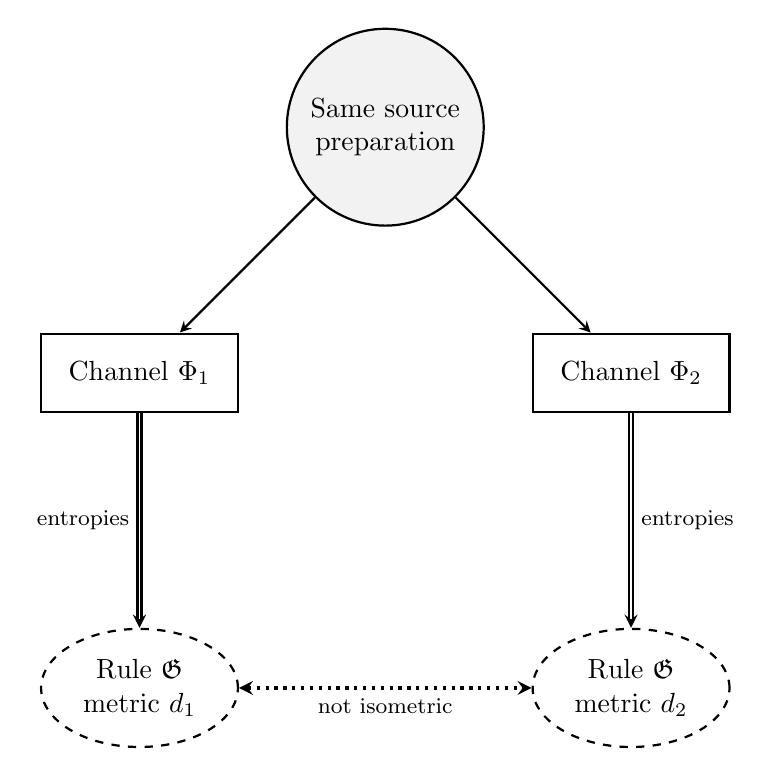
\begin{tikzpicture}[>=stealth, auto, node distance=3cm]
    \tikzstyle{state} = [circle, draw, thick, fill=gray!10, minimum size=2.5cm, align=center]
    \tikzstyle{filter} = [rectangle, draw, thick, fill=white, minimum width=2.5cm, minimum height=1cm, align=center]
    \tikzstyle{geo} = [ellipse, draw, thick, dashed, minimum width=2.5cm, minimum height=1.5cm, align=center]
    \node[state] (Alaya) {Same source\\preparation};
    \node[filter] (Filter1) [below left of=Alaya, xshift=-1cm, yshift=-1cm] {Channel $\Phi_1$};
    \node[filter] (Filter2) [below right of=Alaya, xshift=1cm, yshift=-1cm] {Channel $\Phi_2$};
    \node[geo] (Geo1) [below of=Filter1, yshift=-1cm] {Rule $\mathfrak G$\\metric $d_1$};
    \node[geo] (Geo2) [below of=Filter2, yshift=-1cm] {Rule $\mathfrak G$\\metric $d_2$};
    \draw[->, thick] (Alaya) -- (Filter1);
    \draw[->, thick] (Alaya) -- (Filter2);
    \draw[->, double, thick] (Filter1) -- node[left, font=\footnotesize] {entropies} (Geo1);
    \draw[->, double, thick] (Filter2) -- node[right, font=\footnotesize] {entropies} (Geo2);
    \draw[<->, dotted, very thick] (Geo1) -- node[below, font=\footnotesize] {not isometric} (Geo2);
\end{tikzpicture}
\caption{One global state is reduced by two channels from the same allowed family. The same reconstruction rule turns their entropy data into metrics. The tensor sites and the rule are fixed inputs. Proposition~\ref{prop:ghz} exhibits different diameters; the process-selected sector geometry is a separate construction.}
\label{fig:haff_scheme}
\end{figure}

\section{From relations to spatial structure}
\label{sec:discussion}
\label{sec:spatial-bridge}

\subsection{What the different geometries compare}

The process-selected sectors and the GHZ sites answer different
questions. The first are central atoms of a persistent algebra;
the second are tensor factors supplied to a correlation protocol.
There is no canonical identification between these two sets.
In the rate geometry the channel determines a relation independently
of the input state. In the correlation geometry the state, its
reduction, the site representation and the reconstruction rule all
matter.

A spatial interpretation needs evidence linking these relations to
propagation or intervention. Pure dephasing supplies none of the
required sector transport. A weak Hamiltonian connecting different
sectors is a possible extension, but degenerate blocks generally
retain quantum states that prevent a closed scalar equation for their
populations. Paper~B's protected Bell-pair interaction acts inside a
joint noise sector and does not supply transitions between central
labels \cite{Liu2026PaperB}. Deriving a transfer law would require
its own approximation, error bound and actual intervention ports.

If a reversible transfer process were identified through those
ports, its stationary currents and responses could fix a conductance
form and operational resistance distances. This would give a
distance rule through a stated physical task, as
\eqref{eq:rate-record} does for discrimination. An arbitrary support
of the added Hamiltonian can still encode an arbitrary interaction
graph. Inferring spatial locality, rather than inserting it into
that support, remains the stronger problem.

For a precisely specified response candidate, suppose calibrated
experiments identify a connected reversible jump generator with
rates $q_{ab}$ from $a$ to $b$ and stationary weights $\pi_a>0$.
The response fixes
\[
 \mathcal E(f,f)=\frac12\sum_{a,b}\pi_aq_{ab}(f_b-f_a)^2,\qquad
 \Gamma(f)(a)=\frac12\sum_bq_{ab}(f_b-f_a)^2 .
\]
A possible task convention fixes a reference rate $r_0>0$, with
units $\mathrm{time}^{-1}$, and bounds local quadratic variation:
\begin{equation}
 d_{\Gamma,r_0}(a,b)=\sup\{f_a-f_b:\ \Gamma(f)(c)\le r_0
                           \text{ for all }c\},\qquad f\in\mathbb R^V.
 \label{eq:response-distance}
\end{equation}
On a finite connected graph this is a finite separating metric:
edgewise gradient bounds make every difference bounded, small
multiples of separating functions are feasible, and the supremum
gives the triangle inequality. For dimensionless $f$, this distance
is dimensionless; its conversion to length requires a separate
calibration. The reference rate is part of the task convention.
It is defined here by this task convention; it is not identified
with the effective resistance or asserted to be the sole intrinsic
metric of a jump process. For diffusion forms the energy-measure
analogue defines a standard intrinsic pseudometric, whose
nondegeneracy and agreement with the topology need extra conditions
\cite{Sturm1995}.

\subsection{A same-process locality conjecture}

The world-structure proposal is that the process selecting persistent
organization can also constrain the relations that become spatial.
Selection, record access and propagation should be tested within
one history, rather than supplied by incompatible models.

\begin{conjecture}[Locality from process-selected relations]
\label{conj:process-locality}
There are families of finite carriers, specified by noise and
Hamiltonian operators without assigning their matrix entries to
spatially local gates, for which interaction histories produce
refining persistent block descriptions and calibrated transfer
responses on those blocks. Under refinement these responses admit
a common continuum limit described by a nondegenerate strongly
local Dirichlet form. After calibration, the distances
\eqref{eq:response-distance} converge with these descriptions to
the nondegenerate intrinsic distance of that limit. This distance
is unchanged by alternative descriptions preserving the response,
stationary weights and reference rate.
\end{conjecture}

The conjecture asks for an existence mechanism in one microscopic
family, not a conclusion for every dephasing channel. Its substantial
requirement is the joint formation of stable organization and a
local response limit without a spatial dictionary supplied to the
reconstruction. The finite selection result supplies a persistent-block ingredient; Paper~B's interactions forming protected relations show
that preservation and formation can be distinguished experimentally.
Neither establishes the proposed limit.

A proposed realization must supply the refining blocks, allowed
preparations and readers, measured transfer kernels, limiting form
and its intrinsic distance. It would fail if block dynamics did
not close at the claimed resolution, if persistent long-range
shortcuts prevented a local limit, or if response-preserving
descriptions produced inequivalent limiting distances after common
calibration. Its strongest competing explanation is that any
observed locality was already encoded in the supplied coupling
architecture. A useful realization must show which locality
constraints follow from the history and which remain in that
architecture.

\subsection{Reconstruction and the series}

In holography, extremal-surface areas provide a specific entropy
dictionary \cite{Maldacena1999,RyuTakayanagi2006}; tensor-network
distances use another \cite{Swingle2012}. To infer distinct
spacetimes from separated entropy profiles, a dictionary
$\mathfrak G$ must identify its equivalence relation and satisfy,
for example,
\[
 \mathfrak G[S_1]\simeq_{\rm diff}\mathfrak G[S_2]
       \ \Longrightarrow\ S_1\simeq_{\mathfrak G}S_2 .
\]
This separation property is an input about that dictionary.
Finite readings also require its stability over a confidence
region. The finite model in Section~\ref{sec:geometry} proves
separation under its declared rule rather than assuming a
spacetime dictionary. Imprint's cross-scale analysis asks the related
question of which readable relations survive a change of resolution
and at what cost \cite{LiuImprintRG}.

\begin{conjecture}[Finite permissions approaching geometric access]
\label{conj:finite-geometry}
In a source family with an independently justified local
reconstruction dictionary, histories that enlarge the available
record fragments and calibrate their readout can make the inferred
geometry converge while the generated observable algebra remains
constant. The required growth of visibility, preparation count and
dictionary stability bounds must jointly dominate sampling and
model error.
\end{conjecture}

The finite certificate supplies the mechanism and the costs of this
candidate. For $E$ edges with visibility at least $\nu$, error in
the correlations scales as
$\nu^{-2}\sqrt{\ln(2E/\delta)/n}$ before calibration error.
If reconstructed edge mutual informations have lower bound $\mu$,
distance error carries another factor of order $\mu^{-2}$ times
the number of edges in a shortest path. Consequently, a growing
graph or an approaching zero-information edge can defeat
convergence even while all fixed-algebra labels are unchanged.
The conjecture would fail in a proposed model if its dictionary is
unstable, if common error survives calibration, or if its available
budget cannot overcome these factors. This is a route from finite
permissions to geometric access, not an assumption that a continuum
or its dynamics is already generated.

The spatial/eigenmode example in Appendix~\ref{sec:optional-connectivity}
illustrates dependence of connectivity on factorization. Unlike
Proposition~\ref{prop:ghz}, its empty eigenmode graph has no finite
reconstructed paths.

\section{Conclusion}
\label{sec:conclusion}

A physical process can select an effective organization before
spatial sites have been assigned. In the commuting-noise class,
the organization is a direct sum fixed by the dynamics; its
central sectors and cross-sector coherence rates are intrinsic to
the channel. A finite stability window can select persistent blocks,
and allowed coherent probes identify their rate relation.

What is selected must still be distinguished from what can be
read. Equal system channels can leave different readable records
at a restricted environmental port. Equal entropy functions can
hide operationally incomparable reductions. The qubit criterion
and finite-copy tests make those obstructions quantitative.

The GHZ protocol carries a separate correlation reconstruction
through actual interactions and finite records. Changing the
allocation of a fixed expected flip count changes its certified
metric. Its tensor sites and distance rule remain specified
inputs. Turning process-selected organization into spatial
geometry requires a common account of persistence and actual
transport. Conjecture~\ref{conj:process-locality} states that
remaining mechanism as a testable target within the framework.

\appendix

\section{Proof of the intrinsic window certificate}
\label{app:window-proof}

On a cluster $C$, choose a centre $c$ of its smallest enclosing
ball and put
$B_k=\sum_{a\in C}(u_{a,k}-c_k)P_a$. Scalar shifts do not alter
double commutators. The restricted generator is
\[
 \mathcal L_C(X)=2\Psi(X)-\{R,X\},\qquad
 \Psi(X)=\sum_kB_kXB_k,\qquad R=\sum_kB_k^2 .
\]
Here $\Psi$ is completely positive and
$\|\Psi\|=\|\Psi(I)\|=\|R\|\le r_C^2$.
Thus $\|\mathcal L_C\|\le4r_C^2$. The semigroup is a contraction
on each invariant block, so Duhamel's formula gives
$\|\Phi_t(X)-X\|\le t\kappa_{\rm in}\|X\|$
on $\mathcal B_\pi$.

A strictly containing unital algebra has a nonzero entry between
two different $Q_C$ blocks. Multiplication on both sides by
matrix units already in $\mathcal B_\pi$ isolates a cross-cluster
matrix unit $E_{xy}$. Its loss at time $T$ is
$1-e^{-TD_{ab}}\ge1-e^{-T\Delta_{\rm out}}>\varepsilon$.
Such a containing algebra cannot be stable.

Conversely, any stable block algebra in a common joint eigenbasis
can put $x$ and $y$ together only if
$1-e^{-TD_{ab}}\le\varepsilon$. The separation in
\eqref{eq:intrinsic-window} forbids this across two clusters, so
every stable block of that form lies in one $Q_C$ block.
Two certified partitions therefore refine each other and coincide.

The radii are determined by the Euclidean configuration of $D$.
A computable sufficient upper bound uses the equal-weight centroid:
\[
 \|u_a-\bar u_C\|^2
 =\frac1{|C|}\sum_{b\in C}D_{ab}
   -\frac1{2|C|^2}\sum_{b,c\in C}D_{bc}.
\]
Replacing $r_C^2$ by its largest value over $a\in C$ retains the
certificate. It need not be optimal.

\section{Channel order and entropy tests}
\label{app:entropy-tests}
\subsection{Refinement}

\begin{definition}[Refinement]
\label{def:refine}
For coarse-graining structures $\mathbf c_1,\mathbf c_2$ write $\mathbf c_1\succeq\mathbf c_2$ if there is a CPTP map $\Lambda$ from states on the output space of $\Phi_{\mathbf c_1}$ to states on the output space of $\Phi_{\mathbf c_2}$ with $\Phi_{\mathbf c_2}=\Lambda\circ\Phi_{\mathbf c_1}$. Then $\mathbf c_2$ is a further coarse-graining of $\mathbf c_1$.
\end{definition}

\begin{proposition}[Order on classes]
\label{prop:order}
The relation $\succeq$ is reflexive and transitive but not antisymmetric. Writing $\Phi\sim\Psi$ when each is a post-processing of the other, $\succeq$ induces a partial order on equivalence classes.
\end{proposition}

\begin{proof}
Reflexivity uses $\Lambda=\mathrm{id}$, transitivity uses composition of channels. Two different replacer channels, which output fixed states $\omega_1\ne\omega_2$, simulate each other by a further replacement, so antisymmetry fails. On classes the relation is well defined because composing with a simulating channel does not change membership, and antisymmetry holds by construction.
\end{proof}

If the allowed post-processings are restricted, for example to local, energy-bounded or specified control operations, the restricted class must be closed under composition before the same quotient can be formed. The comparison of channels by approximate post-processing has an operational characterization through success probabilities of discrimination tasks \cite{Jencova2015}; we use only exact post-processing.

\subsection{Mutual information under refinement}

\begin{proposition}[Local and global post-processing]
\label{prop:mi}
For channels $\Lambda_A,\Lambda_B$ acting on $A$ and $B$ separately,
\[
I(A':B')_{(\Lambda_A\otimes\Lambda_B)(\rho)}\le I(A:B)_\rho .
\]
A global CPTP post-processing can increase mutual information: the channel that replaces every two-qubit input by a Bell state takes $|00\rangle$, with $I=0$, to a state with $I=2\ln2$.
\end{proposition}

\begin{proof}
$I(A:B)_\rho=D(\rho_{AB}\Vert\rho_A\otimes\rho_B)$, and $\Lambda_A\otimes\Lambda_B$ maps $\rho_A\otimes\rho_B$ to the product of the new marginals, so data processing for relative entropy gives the inequality. The Bell example is a direct computation.
\end{proof}

A requirement that mutual information decrease under refinement is therefore a theorem for local refinements and false for global ones. A geometric reading of mutual information must say which refinements it allows.

\subsection{Generic separation}

\begin{theorem}[Generic separation for a fixed pair of channels]
\label{thm:inequiv}
Let $\mathcal H$ and $\mathcal K=\mathcal K_A\otimes\mathcal K_{A^c}$ be finite dimensional, and let $\Phi_1\ne\Phi_2$ be CPTP maps from states on $\mathcal H$ to states on $\mathcal K$. The pure inputs on which $\Phi_1$ and $\Phi_2$ agree form a proper real-algebraic subset of Haar measure zero. If, in addition, the real-analytic function
\[
f_A(\Psi):=
S\!\left(\operatorname{Tr}_{A^c}\Phi_1(|\Psi\rangle\!\langle\Psi|)\right)
-S\!\left(\operatorname{Tr}_{A^c}\Phi_2(|\Psi\rangle\!\langle\Psi|)\right)
\]
is not identically zero on each connected component under consideration of the open set where both reduced outputs have full rank, then $f_A(\Psi)\ne0$ for generic inputs in those components.
\end{theorem}

\begin{proof}
Pure-state projectors span the Hermitian operators, so $\Phi_1-\Phi_2$ cannot vanish on all of them. The equality condition is polynomial in the real and imaginary parts of $|\Psi\rangle$, so its solution set is a proper real-algebraic subset and has Haar measure zero. On the full-rank domain the von Neumann entropy, and hence $f_A$, is real analytic, and a nonzero real-analytic function has a zero set of measure zero.
\end{proof}

The nondegeneracy hypothesis cannot be dropped: channels that differ
by a unitary acting on $A$ alone can give different outputs with
identical entropies on every input. Channel inequivalence alone
therefore does not yield an entropic or geometric difference.
Section~\ref{sec:entropy} gives the exact qubit criterion; the tests
below turn its violation into a finite measurement problem.

\subsection{Probes and random inputs}

\begin{corollary}[Nine pure probes and one mixed probe]
\label{cor:probes}
Let the probe set consist of the nine Bloch vectors
\[
\pm e_1,\ \pm e_2,\ \pm e_3,\ (e_1+e_2)/\sqrt2,\ (e_1+e_3)/\sqrt2,\ (e_2+e_3)/\sqrt2 .
\]
If the two channels give equal output entropies on these nine inputs, they give equal output entropies on every pure input. If they also agree at $r=0$, they agree on every input.
\end{corollary}

\begin{proof}
The six axial probes give $b_i=0$ and $A_{ii}+c=0$; the three diagonal probes then give $A_{ij}=0$ for $i\ne j$. This is \eqref{eq:criterion}. At $r=0$, $q=c=-\alpha$, so agreement there gives $\alpha=0$. Then $q$ vanishes on the entire Bloch ball, hence the output lengths and entropies agree everywhere.
\end{proof}

The corollary concerns exact entropy values on nine inputs, not nine measurements. On the unit sphere $q(r)=r^TA_0r+2b^Tr+d$ with $\alpha=\tfrac13\operatorname{tr}A$, $A_0=A-\alpha I$ and $d=c+\alpha$, which is linear in nine real parameters.

\begin{proposition}[Random pure inputs]
\label{prop:haar}
For Haar-random pure inputs,
\begin{equation}
Q:=\mathbb E\,q(r)^2=\frac{2}{15}\|A_0\|_F^2+\frac43\|b\|^2+d^2 .
\label{eq:Q}
\end{equation}
$Q=0$ exactly when \eqref{eq:criterion} holds. If $Q>0$, then $\mathbb E(S_1-S_2)^2\ge Q/4$, and for $0<\tau<1$
\begin{equation}
\Pr\Bigl\{|S_1-S_2|>\tfrac12\sqrt{\tau Q}\Bigr\}
\ge\Pr\{q^2>\tau Q\}
\ge\frac{(1-\tau)Q}{1-\tau Q}.
\label{eq:detect}
\end{equation}
\end{proposition}

\begin{proof}
Use $\mathbb E r_ir_j=\delta_{ij}/3$ and $\mathbb E r_ir_jr_kr_l=(\delta_{ij}\delta_{kl}+\delta_{ik}\delta_{jl}+\delta_{il}\delta_{jk})/15$; odd moments and the cross terms with the traceless $A_0$ vanish. The second claim follows from \eqref{eq:gap-general}. Both outputs are states, so $0\le q^2\le1$; splitting $\mathbb E q^2=Q$ at $q^2=\tau Q$ gives $Q\le\tau Q(1-P)+P$ with $P=\Pr\{q^2>\tau Q\}$, which is \eqref{eq:detect}.
\end{proof}

With $n$ independent Haar inputs, the probability of missing the difference at the level $\tfrac12\sqrt{\tau Q}$ is at most $(1-p_\tau)^n$, where $p_\tau$ is the right side of \eqref{eq:detect}. This assumes exact entropies; the next proposition removes that assumption. The average change of purity over pure inputs is also the basis of the unitarity measure of noise \cite{Wallman2015}; Eq.~\eqref{eq:Q} concerns the difference between two channels rather than the coherence of one.

\subsection{Finitely many copies}

For a qubit, purity and entropy are both monotone functions of the Bloch length, so equal entropy is equivalent to equal purity, and purity can be measured directly. A SWAP test on two copies of a state $\sigma$ returns the outcome $0$ with probability $\tfrac12\bigl(1+\operatorname{Tr}\sigma^2\bigr)$ \cite{Buhrman2001}. For a qubit with Bloch vector $s$ this is $\tfrac34+\tfrac14\|s\|^2$. We assume that every channel use acts on a freshly prepared, known probe state, that the channels do not drift between uses, and that two output copies can be measured jointly.

Finite data cannot establish that the two entropy functions are exactly equal. They can separate equality from a violation of prescribed size, and they can bound how large a violation can be. Put
\[
\kappa_9=\frac{75-3\sqrt{465}}{8}=1.28855\ldots .
\]

\begin{proposition}[Finite-copy test and confidence bound]
\label{prop:finite}
For each of the nine probes $r_k$ of Corollary~\ref{cor:probes}, send $2m$ copies of the input through $\Phi_1$, apply a SWAP test to each of the $m$ output pairs, and do the same for $\Phi_2$. Let $D_k$ be the difference of the two observed frequencies of the outcome $0$.
\begin{enumerate}
\item Given $\gamma>0$, declare the channels different on pure inputs if $\max_k|D_k|>\gamma/8$. If \eqref{eq:criterion} holds, a difference is declared with probability at most $18\,e^{-m\gamma^2/64}$. If $\max_k|q(r_k)|\ge\gamma$, the difference is missed with probability at most $2\,e^{-m\gamma^2/64}$.
\item $\sum_kq(r_k)^2\ge\kappa_9\,Q$, and $\kappa_9$ is the largest constant with this property. Hence $Q\ge Q_0>0$ forces $\max_k|q(r_k)|\ge(\kappa_9Q_0/9)^{1/2}$, and
\[
m\ge\frac{576\,\ln(18/\delta)}{\kappa_9\,Q_0}
\]
output pairs per probe and channel keep both error probabilities below $\delta$ for the hypotheses $Q=0$ and $Q\ge Q_0$.
\item For every $t>0$, with probability at least $1-18\,e^{-mt^2}$,
\[
Q\le\frac{16}{\kappa_9}\sum_{k=1}^9\bigl(|D_k|+t\bigr)^2 .
\]
\end{enumerate}
\end{proposition}

\begin{proof}
The expected value of $D_k$ is $q(r_k)/4$. $D_k$ is a sum of $2m$ independent Bernoulli variables with coefficients $\pm1/m$, so Hoeffding's inequality \cite{Hoeffding1963} gives $\Pr\{|D_k-\mathbb ED_k|\ge t\}\le2e^{-mt^2}$. Under \eqref{eq:criterion} every $\mathbb ED_k$ vanishes, and $t=\gamma/8$ with a union bound over the nine probes gives the first error bound. If $|q(r_k)|\ge\gamma$ for some $k$, then $|\mathbb ED_k|\ge\gamma/4$, and missing it requires $|D_k-\mathbb ED_k|\ge\gamma/8$, which gives the second.

The smallest generalized eigenvalue of the two quadratic forms
$\sum_kq(r_k)^2$ and $Q$ is $\kappa_9$, as computed in
Appendix~\ref{sec:probe-constant}. The largest of nine terms is at least their mean; setting $\gamma^2=\kappa_9Q_0/9$ and requiring $18e^{-m\gamma^2/64}\le\delta$ gives item~2. For item~3, on the event that all nine deviations are at most $t$, which fails with probability at most $18e^{-mt^2}$, we have $|q(r_k)|=4|\mathbb ED_k|\le4(|D_k|+t)$, and $Q\le\kappa_9^{-1}\sum_kq(r_k)^2$.
\end{proof}

If the pure-input criterion is known to hold, the same argument at the mixed probe $r=0$ tests the size of $\alpha$: the expected difference there is $-\alpha/4$, and $m\ge64\ln(2/\delta)/\alpha_0^2$ pairs per channel separate $\alpha=0$ from $|\alpha|\ge\alpha_0$ with error at most $\delta$ in each direction. The pure test uses $18m$ channel uses per channel, $36m$ in all. The constants are conservative. Beyond qubits, purity and entropy are different functionals and this reduction no longer applies.

\subsection{The nine-probe constant}
\label{sec:probe-constant}

On the unit sphere, $\sum_kq(r_k)^2$ and $Q$ are quadratic forms in the nine parameters $(A_0,b,d)$, and both are positive definite; the first because the nine probe values determine the parameters, as in the proof of Corollary~\ref{cor:probes}. Their generalized eigenvalues do not depend on the basis chosen for the parameters, and a direct computation gives the characteristic polynomial, up to a constant factor,
\[
(\lambda-6)\,(4\lambda^2-75\lambda+90)\,(8\lambda^3-225\lambda^2+1620\lambda-2700)^2 .
\]
Its roots are $1.2886$, $2.3962$, $6$, $7.9001$, $17.4614$ and $17.8287$, the three roots of the cubic each counted twice. The smallest is the smaller root of the quadratic factor, $\kappa_9$, and it is attained. 

\section{Record certificate: proof and calibration budgets}
\label{app:record-proof}
\subsection{Proof of Theorem~\ref{thm:record-metric}}
\begin{proof}
Each $Y_iY_j\in[-1,1]$ has expectation $v_iv_jc_{ij}$.
Hoeffding's inequality gives a two-sided tail
$2e^{-n\tau^2/2}$; a union bound covers the $3K$ edge estimates.
The three edges within a run need not be independent.
On the calibration event,
$|v_iv_j-\widehat v_i\widehat v_j|\le2\xi$, by telescoping and the
bounds $v_i,\widehat v_i\le1$. Dividing by
$\widehat v_i\widehat v_j\ge\nu^2$, using $|c_{ij}|\le1$, and
clipping cannot increase the error, proving \eqref{eq:ec}.
The interval construction contains the true mutual informations.
Shortest-path lengths and their diameter are monotone in positive
edge lengths, proving the metric enclosure. Finally
$f'(c)=\operatorname{artanh}c$, so $|\widehat I-I|\le e_I$.
Proposition~\ref{prop:stability}, with three vertices, gives
\eqref{eq:diam-radius}. Each estimated diameter differs from its true
value by at most $R$, so the estimated gap is at least $\Delta-2R$;
two radius-$R$ intervals are disjoint when $\Delta>4R$.
\end{proof}

\subsection{Specified and empirically calibrated readers}
For the equal-flip-count configurations $(.1,.1,.1)$ and
$(.05,.1,.15)$, take one recording qubit per site with overlap
$r_i=.2$. Then $v_i=\sqrt{.96}$ and the correlations lie between
$.56$ and $.72$. With exactly specified $v_i$, use $\nu=\sqrt{.96}$,
$\xi=0$, $\tau=.003$, $b=.8$, $\mu=.16$ and $\delta=.05$.
The choice
\[
n=\left\lceil\frac{2\ln(12/\delta)}{\tau^2}\right\rceil
  =1\,217\,920
\]
runs per configuration gives $e_c=.003125$,
$e_I=.0034332$ and $R<.275$.
The true diameter gap is $1.505919931>4R$.
Thus a finite record-only experiment separates the two geometries
with confidence at least $.95$, under the stated source and apparatus
model. The sample bound is conservative and does not claim optimal
tomography.

A known unitary specification is not free empirical calibration.
If the $v_i$ are unknown, prepare reference sources in $Z=+1$ and
apply the same record couplings and readers. Each reference outcome
has mean $v_i$. For $N$ independent reference runs per site,
clipping the empirical mean to $[0,1]$ yields
\[
\Pr\{\max_i|\widehat v_i-v_i|>\xi\}
   \le6e^{-N\xi^2/2}
\]
for three shared readers; separately calibrated readers for $K$
configurations replace $6$ by $6K$. Thus $N\ge\lceil2\ln(6/\delta_{\rm cal})/\xi^2\rceil$ per site
suffices. Reject calibrations below $\nu$.
For the same two geometries, take $\xi=.001$,
$\delta_{\rm cal}=.025$, $\nu=.978$ and $\tau=.002$.
Then $N=10\,961\,278$ reference runs per site and
$n=3\,086\,894$ main runs per configuration give total failure
at most $.05$, $e_c<.004182$, $R<.36955$ and $4R<1.4782<\Delta$.
On the calibration event the true $v_i=\sqrt{.96}$ ensures
$\widehat v_i>\nu$; the correlation bound also stays inside $b=.8$.
The reference budget is therefore $3N$ additional preparations and
readouts, not part of the $2n$ main runs.
Equation~\eqref{eq:ec} includes their residual error. Prepared
reference pointers, their basis labels and the stability of the
reader between calibration and use are additional physical resources.

The comparison uses $2n$ preparations of the same GHZ source,
$6n$ fresh noise ancillas, $6n$ fresh recording qubits, $6n$ local
binary readouts and communication of the outcomes to a comparator,
plus any calibration runs. The expected noise-flip count is $.3$
per source in both configurations; their recording and readout
schedule is identical. Preparation, switching work, storage,
communication and renewal do not vanish because the counts agree.
No heat or total-energy equality follows from the flip count, and
this finite protocol supplies no reservoir reset.

\section{No canonical tensor factorization}
\label{sec:nopref}

For a Hilbert space $\mathcal H_{\mathrm{total}}$ of dimension $d_Ad_B$ with $d_A,d_B>1$, there is no unique way to write $\mathcal H_{\mathrm{total}}=\mathcal H_A\otimes\mathcal H_B$ without further physical input. Given any pure state $|\Psi_U\rangle$, choose a unitary $U$ with $U(|0\rangle_A\otimes|0\rangle_B)=|\Psi_U\rangle$ and pull the reference factors through $U$; in the resulting factorization $|\Psi_U\rangle$ is a product. More generally, observables can be chosen so that a given pure state has any prescribed Schmidt decomposition \cite{HarshmanRanade2011}.

What survives is typicality for a family of factorizations fixed in advance.

\begin{theorem}[Entanglement typicality for a specified family]
\label{thm:nofact}
Let $\mathcal H_{\mathrm{total}}$ be finite dimensional and let
$\mathfrak F=\{\mathbf f_1,\ldots,\mathbf f_m\}$ be a finite family of
nontrivial tensor factorizations selected by a physical rule that does not depend on the sampled state.  Write
$\mathcal H_{\mathrm{total}}=\mathcal H_{A_j}\otimes\mathcal H_{B_j}$
with $d_{A_j}\le d_{B_j}$.  For $\delta>0$ let
\[
p_j(\delta):=
\Pr_{\Psi\sim\mathrm{Haar}}
\left[S(\rho_{A_j})<\log d_{A_j}-\delta\right].
\]
Then
\[
\Pr\left[
S(\rho_{A_j})\ge\log d_{A_j}-\delta
\text{ for every }j
\right]
\ge 1-\sum_{j=1}^m p_j(\delta),
\]
and standard concentration estimates make each $p_j(\delta)$ small at large dimension under the usual conditions on the dimension ratio.
\end{theorem}

\begin{proof}
For each fixed $\mathbf f_j$, Page's formula gives~\cite{Page1993}
\begin{equation}
\label{eq:page}
\mathbb{E}[S(\rho_{A_j})]
=\sum_{k=d_{B_j}+1}^{d_{A_j}d_{B_j}}\frac1k
-\frac{d_{A_j}-1}{2d_{B_j}},
\end{equation}
and concentration of measure bounds the lower tail~\cite{HaydenLeungWinter2006}; this tail is $p_j(\delta)$.  The union bound over the finite, preselected family proves the inequality.
\end{proof}

The size of the statement matters. For a balanced split $d_A=d_B$, Eq.~\eqref{eq:page} gives a mean entropy of $\log d_A-\tfrac12+o(1)$, so typical states are close to maximally entangled but keep a gap of about half a nat. Drawing the factorization at random with the state fixed is equivalent to drawing the state at random with the factorization fixed. Hence for a fixed state, product factorizations form a set of measure zero, while factorizations with small but nonzero entanglement have small positive measure.

Theorem~\ref{thm:nofact} says nothing about all factorizations and does not pick out any member of $\mathfrak F$. Which family is admissible, and why, is a question of quantum mereology \cite{Cotler2019,CarrollSingh2021}. Earlier work showed that subsystem structure is induced by the accessible observables rather than given by the Hilbert space \cite{Zanardi2001,Zanardi2004}. The channel-level results in the main text retain the accessible-observable view while distinguishing its algebra from its resolution.

\section{Other connectivity constructions}\label{sec:optional-connectivity}

When a metric on a parameter space of coarse-grained states is wanted, the finite-dimensional construction is the quantum Fisher metric. For a smooth faithful family $\lambda\mapsto\rho_{\mathbf c}(\lambda)$, define the symmetric logarithmic derivatives by $\partial_a\rho_{\mathbf c}=\tfrac12(L_a\rho_{\mathbf c}+\rho_{\mathbf c}L_a)$ and
\begin{equation}
g^{\mathrm{QF}}_{ab}(\lambda)
:=\frac12\operatorname{Tr}\!\left[
\rho_{\mathbf c}(\lambda)\{L_a,L_b\}\right].
\label{eq:qfim}
\end{equation}
This is a positive-semidefinite Riemannian metric on identifiable parameter directions \cite{Petz1996}. It is not a Lorentzian spacetime metric, and the pairwise numbers $\mu_{\mathbf c}(A,B)$ do not determine it without an additional map from graph or state parameters to geometry.

\subsection{Spatial and eigenmode descriptions of a free-fermion chain}

\begin{example}[A dimerized free-fermion chain]
\label{ex:fermion}
Take a periodic chain of $2L$ sites with alternating hopping amplitudes $t_1=1$ and $t_2=1/2$,
\[
H=-\sum_{c=0}^{L-1}\bigl(t_1\,c_{2c}^\dagger c_{2c+1}+t_2\,c_{2c+1}^\dagger c_{2c+2}+\mathrm{h.c.}\bigr),
\]
at half filling. The single-particle spectrum has two bands separated by the gap $2|t_1-t_2|=1$, and the ground state fills the lower band, $|\Psi_0\rangle=\prod_k a_{k,-}^\dagger|0\rangle$, where $a_{k,-}$ are the lower-band Bloch modes. In the description by occupation numbers of the band-resolved Bloch modes the ground state is a product of filled and empty modes: every set of modes has a pure reduced state, disjoint sets have zero mutual information, and the connectivity graph is empty. In the spatial description blocks of sites are correlated. For $L=60$ and blocks of four sites, the block entropy saturates at $.3554$ as the block grows, as the area law for gapped one-dimensional systems requires \cite{Hastings2007,Eisert2010}. The mutual information between two blocks falls from $.333$ for adjacent blocks to $9.0\times10^{-5}$ at a separation of ten sites and $5.2\times10^{-8}$ at twenty, close to $e^{-r/1.32}$. The connectivity graph is dominated by edges between neighbouring blocks.
\end{example}

The second description has to be chosen with care. Plain Fourier modes are not enough when the Hamiltonian is not translation invariant: for two disconnected dimers on four sites, $H=-(c_0^\dagger c_1+c_2^\dagger c_3+\mathrm{h.c.})$ at half filling, the gap at fixed particle number is $2$, yet the Fourier modes $k=\pi/2$ and $3\pi/2$ share one particle in superposition and have mutual information $2\ln2$. A translation-invariant single-band chain with particle conservation is gapless unless its band is full or empty, so a gapped example whose ground state is a product of mode occupations needs band-resolved modes, as above, or in general the single-particle eigenmodes of the Hamiltonian.

The example shows that connectivity depends on the factorization: the spatial description has short-range edges and the eigenmode description has none. It does not exhibit two reconstructed geometries, since its zero-connectivity graph supplies no finite paths under the chosen rule; Proposition~\ref{prop:ghz} is the example in which both descriptions produce geometries.


\begin{thebibliography}{99}

\bibitem{Zurek2003}
W. H. Zurek, \emph{Decoherence, einselection, and the quantum origins of the classical}, Rev. Mod. Phys. \textbf{75}, 715 (2003).

\bibitem{Maldacena1999}
J. M. Maldacena, \emph{The Large N limit of superconformal field theories and supergravity}, Int. J. Theor. Phys. \textbf{38}, 1113 (1999).

\bibitem{VanRaamsdonk2010}
M. Van Raamsdonk, \emph{Building up spacetime with quantum entanglement}, Gen. Relativ. Gravit. \textbf{42}, 2323 (2010).

\bibitem{RyuTakayanagi2006}
S. Ryu and T. Takayanagi, \emph{Holographic Derivation of Entanglement Entropy from AdS/CFT}, Phys. Rev. Lett. \textbf{96}, 181602 (2006).

\bibitem{Zanardi2001}
P. Zanardi, \emph{Virtual Quantum Subsystems}, Phys. Rev. Lett. \textbf{87}, 077901 (2001).

\bibitem{Zanardi2004}
P. Zanardi, D. A. Lidar, and S. Lloyd, \emph{Quantum Tensor Product Structures are Observable Induced}, Phys. Rev. Lett. \textbf{92}, 060402 (2004).

\bibitem{Viola2004}
H. Barnum, E. Knill, G. Ortiz, R. Somma, and L. Viola, \emph{A Subsystem-Independent Generalization of Entanglement}, Phys. Rev. Lett. \textbf{92}, 107902 (2004).

\bibitem{HarshmanRanade2011}
N. L. Harshman and K. S. Ranade, \emph{Observables can be tailored to change the entanglement of any pure state}, Phys. Rev. A \textbf{84}, 012303 (2011), arXiv:1102.0955.

\bibitem{Haag1996}
R. Haag, \emph{Local Quantum Physics: Fields, Particles, Algebras}, Springer-Verlag (1996).

\bibitem{Page1993}
D. N. Page, \emph{Average entropy of a subsystem}, Phys. Rev. Lett. \textbf{71}, 1291 (1993).

\bibitem{HaydenLeungWinter2006}
P.~Hayden, D.~W.~Leung, and A.~Winter,
\emph{Aspects of generic entanglement},
Commun.\ Math.\ Phys.\ \textbf{265}, 95--117 (2006).

\bibitem{Cotler2019}
J.~Cotler, G.~Penington, and D.~H.~Ranard,
\emph{Locality from the spectrum},
Commun.\ Math.\ Phys.\ \textbf{368}, 1267--1296 (2019).

\bibitem{CarrollSingh2021}
S.~M.~Carroll and A.~Singh,
\emph{Quantum mereology: Factorizing Hilbert space into subsystems with quasiclassical dynamics},
Phys.\ Rev.\ A \textbf{103}, 022213 (2021).

\bibitem{Jencova2015}
A. Jen\v{c}ov\'a, \emph{Comparison of quantum channels and statistical experiments}, arXiv:1512.07016 (2015).

\bibitem{RuskaiSzarekWerner2002}
M. B. Ruskai, S. Szarek, and E. Werner, \emph{An analysis of completely-positive trace-preserving maps on $\mathcal M_2$}, Linear Algebra Appl. \textbf{347}, 159--187 (2002), arXiv:quant-ph/0101003.

\bibitem{FujiwaraAlgoet1999}
A. Fujiwara and P. Algoet, \emph{One-to-one parametrization of quantum channels}, Phys. Rev. A \textbf{59}, 3290 (1999).

\bibitem{Wallman2015}
J. Wallman, C. Granade, R. Harper, and S. T. Flammia, \emph{Estimating the coherence of noise}, New J. Phys. \textbf{17}, 113020 (2015), arXiv:1503.07865.

\bibitem{Buhrman2001}
H. Buhrman, R. Cleve, J. Watrous, and R. de Wolf, \emph{Quantum fingerprinting}, Phys. Rev. Lett. \textbf{87}, 167902 (2001), arXiv:quant-ph/0102001.

\bibitem{Helstrom1976}
C.~W.~Helstrom, \emph{Quantum Detection and Estimation Theory},
Academic Press (1976).

\bibitem{Hoeffding1963}
W. Hoeffding, \emph{Probability inequalities for sums of bounded random variables}, J. Amer. Statist. Assoc. \textbf{58}, 13--30 (1963).

\bibitem{Petz1996}
D. Petz, \emph{Monotone metrics on matrix spaces}, Linear Algebra Appl. \textbf{244}, 81 (1996).

\bibitem{Swingle2012}
B. Swingle, \emph{Entanglement Renormalization and Holography}, Phys. Rev. D \textbf{86}, 065007 (2012).

\bibitem{Eisert2010}
J.~Eisert, M.~Cramer, and M.~B.~Plenio,
\emph{Colloquium: Area laws for the entanglement entropy},
Rev.\ Mod.\ Phys.\ \textbf{82}, 277 (2010).

\bibitem{Hastings2007}
M.~B.~Hastings,
\emph{An area law for one-dimensional quantum systems},
J.\ Stat.\ Mech.\ \textbf{2007}, P08024 (2007),
arXiv:0705.2024.

\bibitem{Liu2026PaperB}
S.~Liu, \emph{Coupling, Records, and Stable Relations: Formation, Protected Content and the Lifetime of a Geometry}, Zenodo (2026), DOI: 10.5281/zenodo.18367060.

\bibitem{Liu2026PaperE}
S.~Liu, \emph{Measurement as Accessibility: Measurement Permissions, Stable Records and Public Readout}, Zenodo (2026), DOI: 10.5281/zenodo.18400065.

\bibitem{LiuImprintRG}
S.~Liu, \emph{Renormalization and Imprint Filtering: Source Identification, Memory, and Calibration}, Zenodo (2026), DOI: 10.5281/zenodo.20151451.

\bibitem{Fagnola2019}
F.~Fagnola, J.~E.~Gough, H.~I.~Nurdin and L.~Viola,
\emph{Mathematical Models of Markovian Dephasing},
arXiv:1811.11784 (2019).

\bibitem{LiuFoundationI}
S.~Liu, \emph{Foundation I: From Source to Manifestation.
Accessible Algebras from a Source, Its Noise and a Readable Seed}, Zenodo (2026).

\bibitem{Sturm1995}
K.-T.~Sturm, \emph{On the geometry defined by Dirichlet forms},
in \emph{Seminar on Stochastic Analysis, Random Fields and
Applications}, Progress in Probability \textbf{36},
231--242 (1995).

\end{thebibliography}

\end{document}
